\documentclass[a4paper,12pt]{article}
\usepackage{amsmath,amsfonts,amssymb}
\usepackage{tikz}
\usepackage{geometry}
\geometry{margin=1in}

\title{Sine Law\\Explained}
\author{Tutoring Centre Ferndale\\

\includegraphics[width=4em]{ApS_logo.png}}
\date{}

\begin{document}

\maketitle

The sine law states:
\[
\frac{a}{\sin A} = \frac{b}{\sin B} = \frac{c}{\sin C} = 2r,
\]
where \(r\) is the radius of the circumscribed circle around a triangle. This law establishes a relationship between the sides of a triangle, the angles opposite those sides, and the circle that passes through the triangle's vertices.\\

Given a triangle \(\triangle ABC\), its circumscribed circle centered at \(O\), and the isosceles triangle \(\triangle OBC\). Let \(M\) be the midpoint of \(BC\). The segment \(OM\) is perpendicular to \(BC\), making \(\triangle OMB\) a right triangle.

\begin{center}
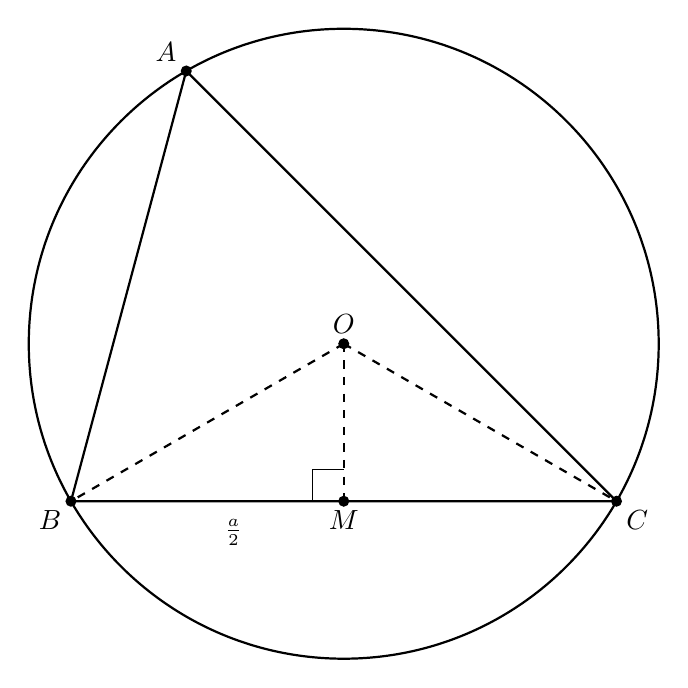
\begin{tikzpicture}[scale=2]
    \draw[thick] (0,0) circle(2);
    \coordinate (O) at (0,0); % Circle center
    \coordinate (A) at (120:2); % Point A
    \coordinate (B) at (210:2); % Point B
    \coordinate (C) at (-30:2); % Point C
    \coordinate (M) at (0,-1); % Midpoint of BC
    \draw[thick] (A) -- (B) -- (C) -- cycle;
    \draw[thick,dashed] (O) -- (B);
    \draw[thick,dashed] (O) -- (C);
    \draw[thick,dashed] (O) -- (M);
    \fill (A) circle(1pt) node[above left] {$A$};
    \fill (B) circle(1pt) node[below left] {$B$};
    \fill (C) circle(1pt) node[below right] {$C$};
    \fill (O) circle(1pt) node[above] {$O$};
    \fill (M) circle(1pt) node[below] {$M$};
    \draw (-0.2,-1) -- (-0.2,-0.8) -- (0,-0.8);
    \node at (-0.7,-1.2) {\small $\frac{a}{2}$};
\end{tikzpicture}
\end{center}

\newpage

\begin{itemize}
\item By the definition of sine:
\[
\sin \angle BOM = \frac{\text{opposite}}{\text{hypotenuse}} = \frac{BM}{OB} = \frac{a/2}{r} = \frac{a}{2r}.
\]
\end{itemize}

"The central angle is twice the inscribed angle" is a fundamental property of circles. It means that for a given arc of a circle, the angle subtended by that arc at the center of the circle (called the central angle) is twice the angle subtended by the same arc at any point on the circle's circumference (called the inscribed angle).\\

\begin{itemize}
\item The angle subtended by \(BC\) at the center of the circle is \(2\angle A\).
\item Therefore, \(\angle BOM = \angle A\).
\end{itemize}

\begin{itemize}
\item Substituting \(\angle BOM = \angle A\) into the sine expression gives:
       \[
       \sin \angle A = \frac{a}{2r}.
       \]
\item Rearranging, we find:
       \[
       \frac{a}{\sin A} = 2r.
       \]
\end{itemize}

This reasoning applies similarly to the other sides and angles of the triangle, resulting in the full sine law.

\end{document}
